\section{Introduction}

The typical running pattern for scientific application referring to simulation, analyzing and visualization tasks are divided into post-processing and in-situ\cite{childs2012situ}. Post-processing use disk or memory staging service to transfer the intermediate data. In-situ processing is a different approach to solve the gap between the computation and communication performance of HPC infrastructure without involving disk storage\cite{childs2012situ}. Several works are focusing on the in-situ pattern and how to leverage the scientific application\cite{bauer2016situ,oldfield2014evaluation} by the in-situ pattern. Figure 1 shows the typical scientific workflow pattern.

\begin{figure} 
\centering
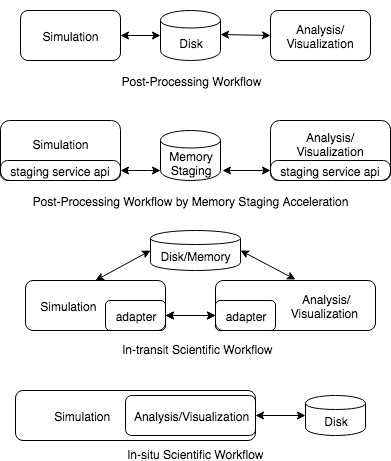
\includegraphics[width=0.75\linewidth]{./figure/scientificworkflowpattern.jpg}
\caption{Scientific Workflow Pattern}
 \label{fg:state}
\end{figure} 


The main task of scientific workflow aims to solve the problems of how and when to run the task in an automatic way as far as possible. Post-processing can be supported well by workflow based DAG (Directed Acyclic Graph) with fixed dependency before workflow run. Even though there are all kinds of work focusing on the intermediate component such as data staging service or in-situ adaptor to leverage specific scenarios (we will discuss this in Background and related work) there are few works explore how to support hybrid pattern in portable, flexible and scalable way(the aim of the experiments). For example, we could use the in-situ part in the simulation to identify if some interesting things happen, if the interesting happens, the in-transit pattern can be used to notify analysis, analysis and visualization component to load data from staging service can be triggered at the same time. 

One challenge for scientific workflow is how to support the complex integration of application patterns including in-situ, in-transit and post-processing tasks\cite{oldfield2014evaluation}. There are two questions needed to be solved in this scenario. (1) Tasks in a workflow is not in same abstraction level, for example, the in-situ part can be a thread in a program and the post-processing part is another program (2) When to run task is unknown before workflow start, the task could be triggered several times or even not be triggered based on the content of intermediate data application.

Our work provides a method based on event programming to leverage the hybrid scientific pattern including in-situ and in-transit pattern, we also implement an event driving workflow tool to compose the scientific application and evaluate its effectiveness in experiment part. The main advantages of this event-driven workflow include:

(1)The dependency could be defined in a more flexible form based on execution sequence or content of intermediate data.

(2)The workflow tool could help the user to express the dependency and control for tasks with different abstraction level and running pattern such as in-situ, in-transit and post-processing.

(3)There is also potential to combine this workflow with low-level resource scheduler system to leverage whole running task of the scientific workflow (more detailed after experiments finishing, maybe provide some good practice to implement the hybrid workflow including in-situ in-transit and post-processing)

The rest paper is organized as follows, Section \uppercase\expandafter{\romannumeral2} introduce the background and the related work of event-driven workflow, Section \uppercase\expandafter{\romannumeral3} introduce the design and implementation of workflow framework. Section \uppercase\expandafter{\romannumeral4} presents the experiments to show the performance and effectiveness of the framework. Section \uppercase\expandafter{\romannumeral5} introduce the conclusion and the future work of the work.
